\documentclass[aspectratio=43]{beamer}
% Packages
\usepackage{amsmath,amssymb,amsfonts}
\usepackage{bm}
\usepackage{mathtools}

% Colors
\definecolor{MITBlue}{RGB}{57,55,177}

% Beamer settings
\setbeamertemplate{navigation symbols}{}

\setbeamertemplate{footline}{
    \leavevmode%
    \hbox{%
        \begin{beamercolorbox}[
            wd=.85\paperwidth,
            ht=2.5ex,
            dp=1.2ex,
            leftskip=1cm
        ]{author in head/foot}
            \tiny Internship Report Dibyanshu Shekhar Dey 25EC64R23
        \end{beamercolorbox}%
        \begin{beamercolorbox}[
            wd=.15\paperwidth,
            ht=2.5ex,
            dp=1.2ex,
            center
        ]{date in head/foot}
            \tiny\insertframenumber
        \end{beamercolorbox}%
    }%
}

% Frame title
\setbeamertemplate{frametitle}{
    \vspace{-0.15cm}
    \nointerlineskip
    \begin{beamercolorbox}[
        wd=\paperwidth,
        ht=0.65cm,
        dp=0.15cm,
        leftskip=0.3cm
    ]{frametitle}
        \usebeamerfont{frametitle}
        \insertframetitle
    \end{beamercolorbox}
}

\setbeamercolor{frametitle}{fg=white,bg=MITBlue}
\setbeamerfont{frametitle}{size=\large,series=\normalfont}
% Body
\setbeamercolor{normal text}{fg=black,bg=white}
\setbeamercolor{structure}{fg=MITBlue}
\setbeamerfont{normal text}{size=\normalsize}

% Title page
\setbeamertemplate{title page}{
    \begin{center}
        \vspace{0.5cm}
        \begin{beamercolorbox}[
            wd=0.82\paperwidth,
            ht=1.25cm,
            center
        ]{title}
            \color{white}
            \usebeamerfont{title}
            \inserttitle
        \end{beamercolorbox}
        \vspace{0.7cm}
        {\large\insertauthor}
        \vspace{0.3cm}
        {\normalsize\insertinstitute}

    \end{center}
}

\setbeamercolor{title}{
    bg=MITBlue
}

\setbeamerfont{title}{
    size=\large,
    series=\bfseries
}

% Document
\title{Internship Report\\[2mm]Score Matching techniques on Goodness-of-Fit tests}
% \author{Dibyanshu Shekhar Dey\\[2mm]
% 25EC64R23}
% \vspace{0.1cm}
% \institute{Dept of EECE\\
% IIT Kharagpur}
\author{
    Dibyanshu Shekhar Dey\\[2mm]
    25EC64R23\\[5mm]
    Dept. of EECE\\[2mm]
    IIT Kharagpur\\[5mm]
    2 September 2026
}


\date{2 September 2026}
\begin{document}

\begin{frame}
    \titlepage
\end{frame}


%slide 2
\begin{frame}{Motivation \& Objectives}
\begin{center}
\textcolor{MITBlue}{\large Goodness-of-Fit Testing}
\vspace{0.1cm}
High-dimensional data and images
\vspace{0.1cm}
KSD requires the score function
\[s_q(x)=\nabla_x \log q(x)\]
\vspace{0.1cm}
\textcolor{MITBlue}{\textbf{Learn the score using Score Matching}}
\end{center}
\vspace{0.1cm}
\textbf{Objectives}
\begin{itemize}
    \item Evaluate KSD-U on toy Gaussian distributions.
    \item Combine Score Matching with KSD for MNIST.
    \item Generate samples using Diffusion Posterior Sampling.
    \item Apply KSD to the generated samples.
\end{itemize}
\end{frame}

% slide 3
\begin{frame}{Kernelized Stein Discrepancy - I}

\textbf{Goodness-of-Fit problem:}

\[
H_0:p=q
\qquad\text{vs.}\qquad
H_1:p\neq q
\]

\vspace{0.2cm}

Given samples $x_i\sim p(x)$ and the reference score

\[
s_q(x)=\nabla_x\log q(x),
\]

KSD measures the discrepancy between the unknown distribution
$p$ and the reference distribution $q$.

\vspace{0.2cm}

\textbf{KSD-U statistic:}

\[
\boxed{
\widehat{S}_u(p,q)
=
\frac{1}{n(n-1)}
\sum_{i\neq j}u_q(x_i,x_j)
}
\]

where $u_q(x_i,x_j)$ is the kernelized Stein kernel.
\end{frame}

%slide 4
\begin{frame}{Kernelized Stein Discrepancy - II}
where
\[
\begin{aligned}
u_q(x,x')={}&
s_q(x)^\top k(x,x')s_q(x')
+s_q(x)^\top\nabla_{x'}k(x,x')\\
&+\nabla_x k(x,x')^\top s_q(x')
+\operatorname{tr}\left(\nabla_{x,x'}k(x,x')\right).
\end{aligned}
\]

\vspace{0.15cm}
\textbf{RBF kernel:}
\[
k(x,x')
=
\exp\left(
-\frac{\|x-x'\|^2}{2h^2}
\right),
\qquad
\boxed{h=\sqrt{\frac{D}{2}}}
\]

\vspace{0.15cm}
\textbf{Hypothesis test:}
Bootstrap the KSD-U statistic and reject $H_0$ when the
observed statistic is sufficiently large.
\end{frame}

%slide 5
\begin{frame}{KSD: Toy Experiments - I}

\textbf{Experimental setup}

\[
H_0:X\sim\mathcal{N}(0,\sigma^2)
\qquad\text{vs.}\qquad
H_1:X\sim\mathcal{N}(\delta,\sigma^2)
\]

\begin{itemize}
    \item Vary the mean $\delta$ or variance $\sigma$ of the alternative.
    \item Evaluate the KSD-U bootstrap test using ROC, AUC and error rate.
\end{itemize}

\vspace{0.15cm}

\begin{center}
    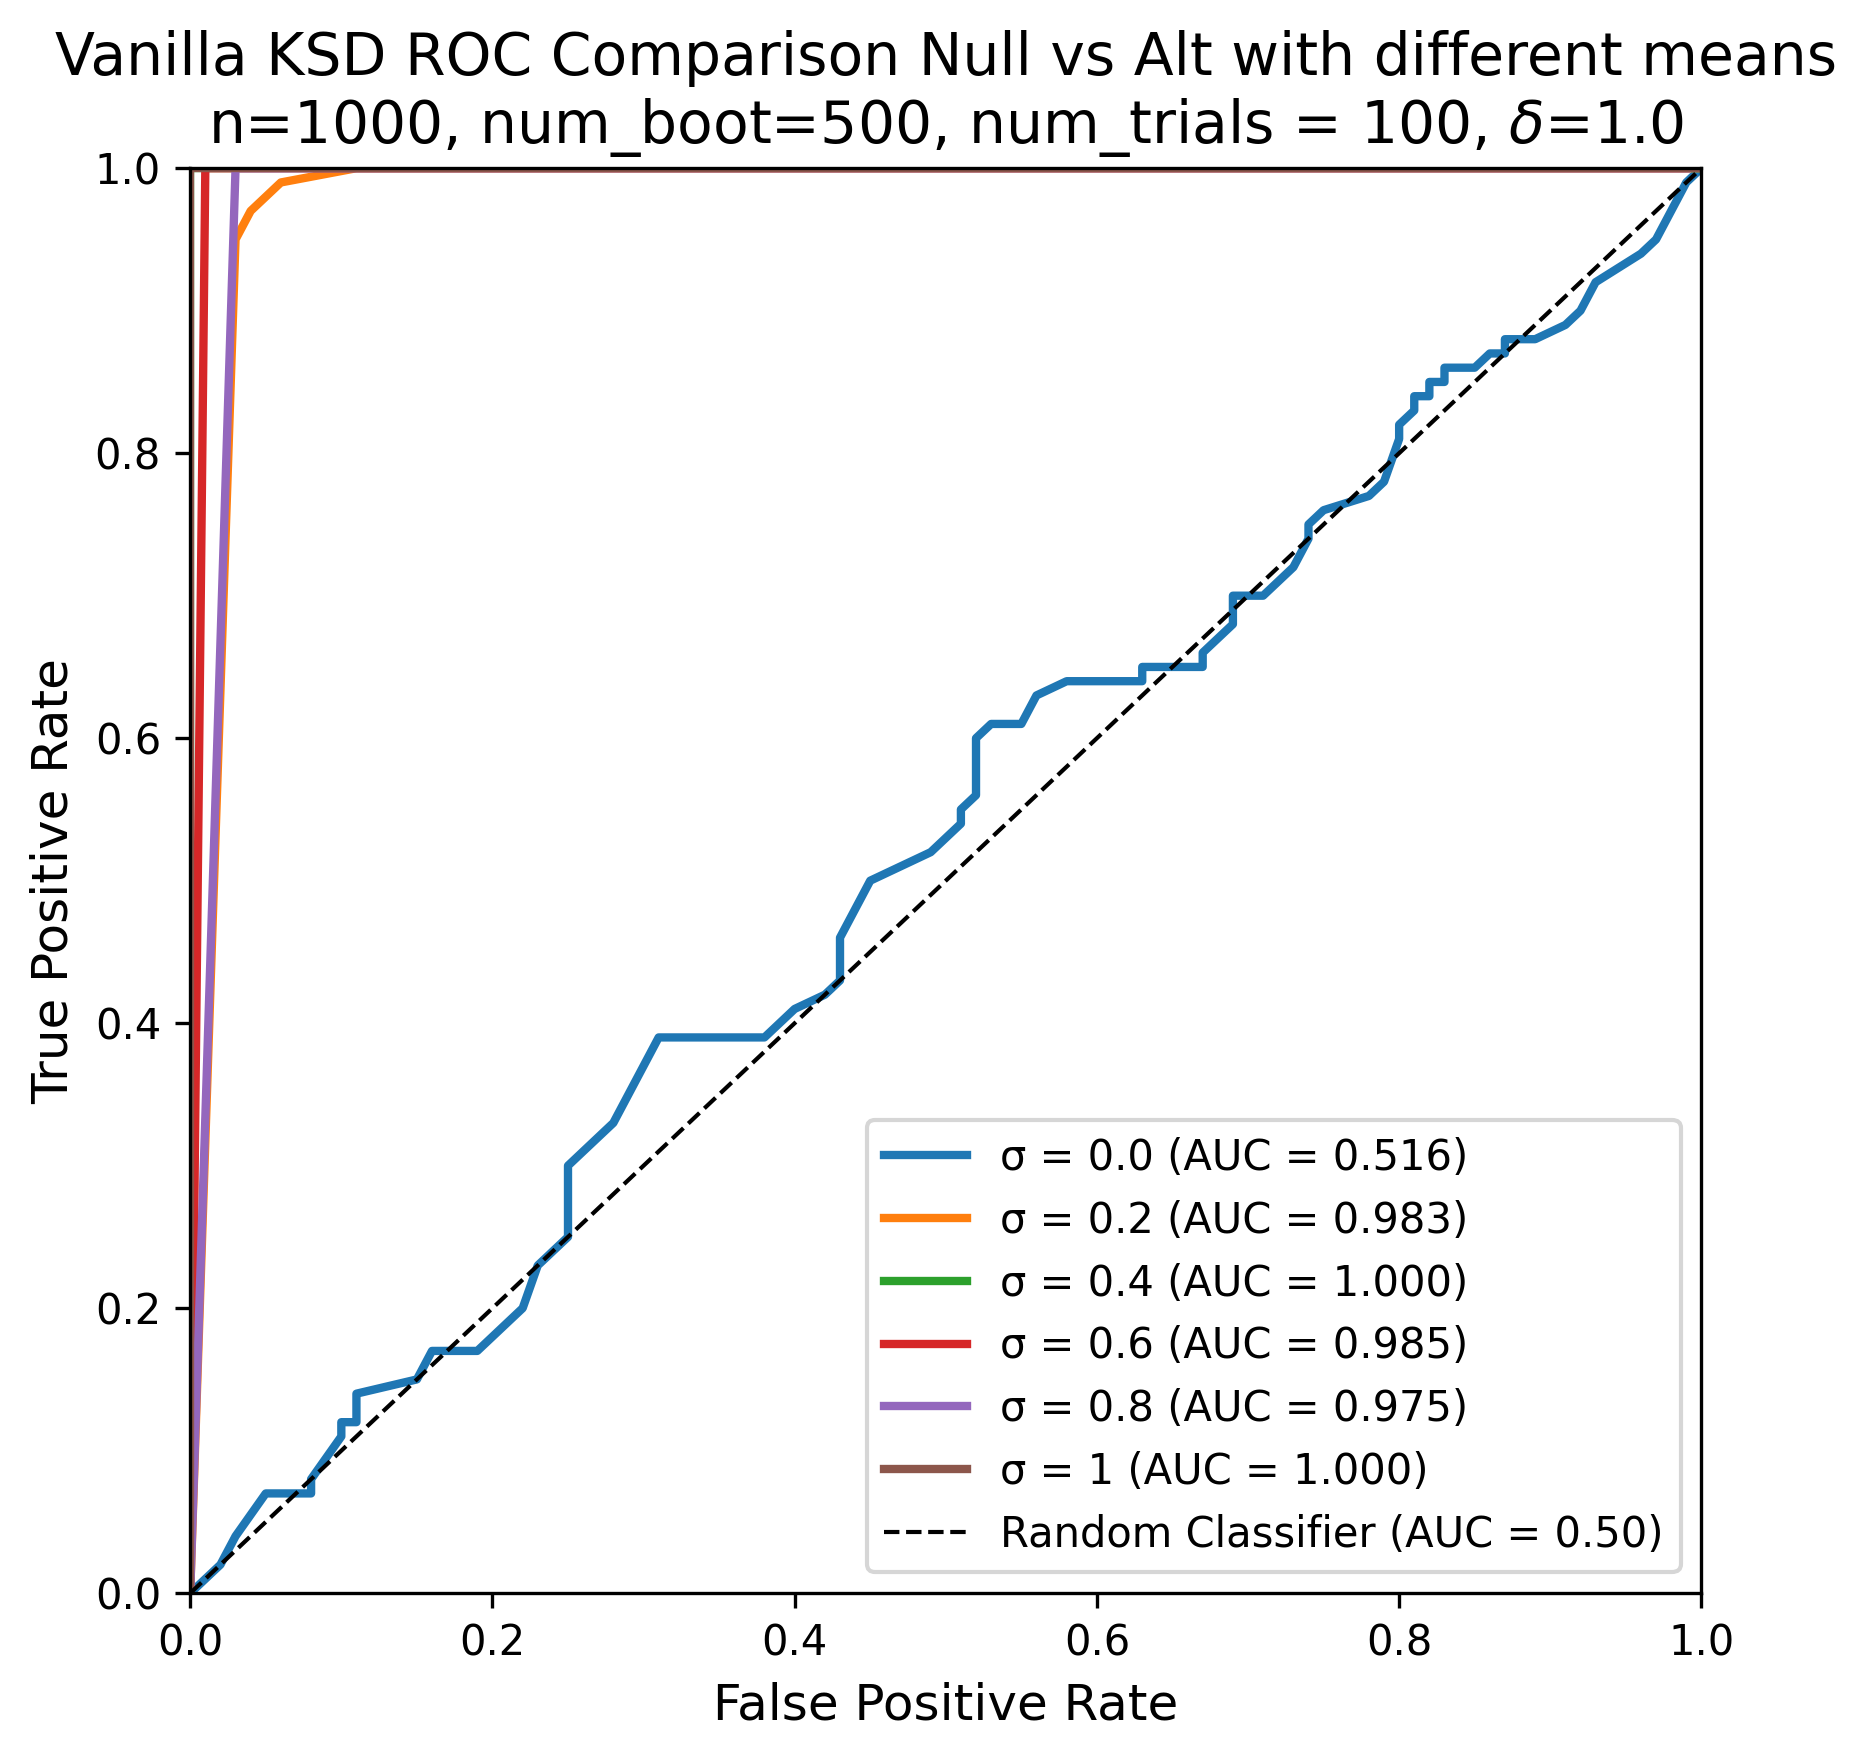
\includegraphics[width=0.47\textwidth]{KSD/Vanilla/vanilla_ksd_roc_comparison_different_deltas.png}
    \hspace{0.02\textwidth}
    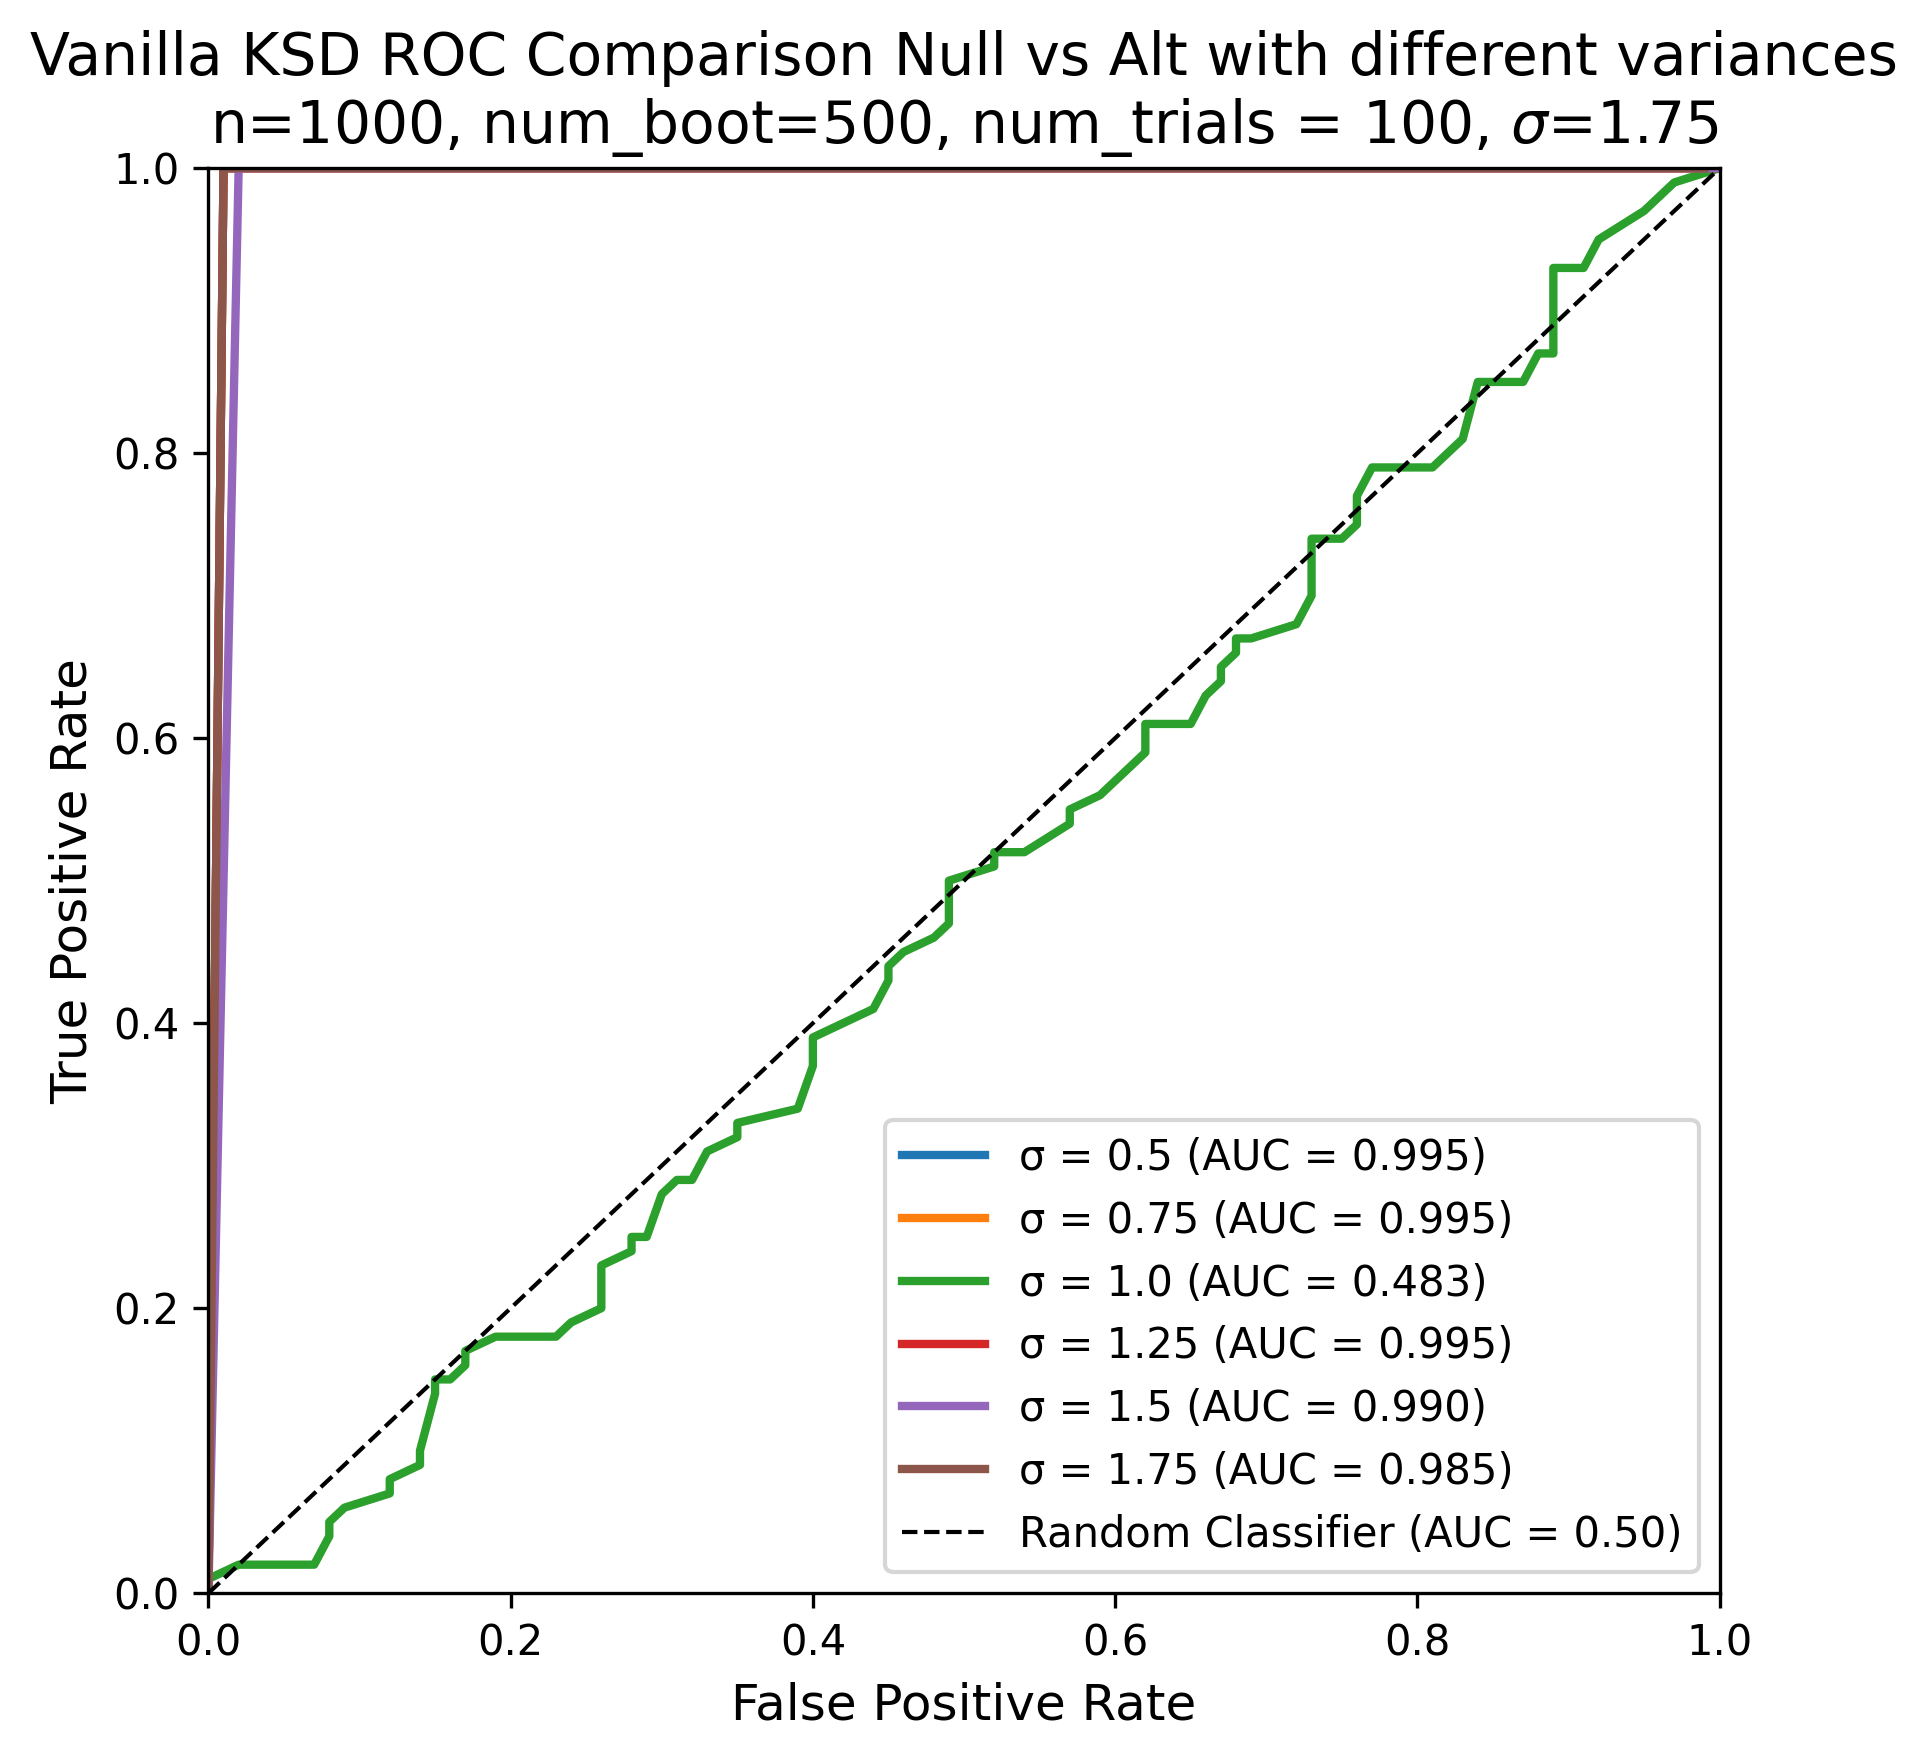
\includegraphics[width=0.47\textwidth]{KSD/Vanilla/vanilla_ksd_roc_comparison_different_sigmas.png}
\end{center}

\end{frame}

\begin{frame}{KSD: Toy Experiments - II}
\begin{center}

\begin{center}
    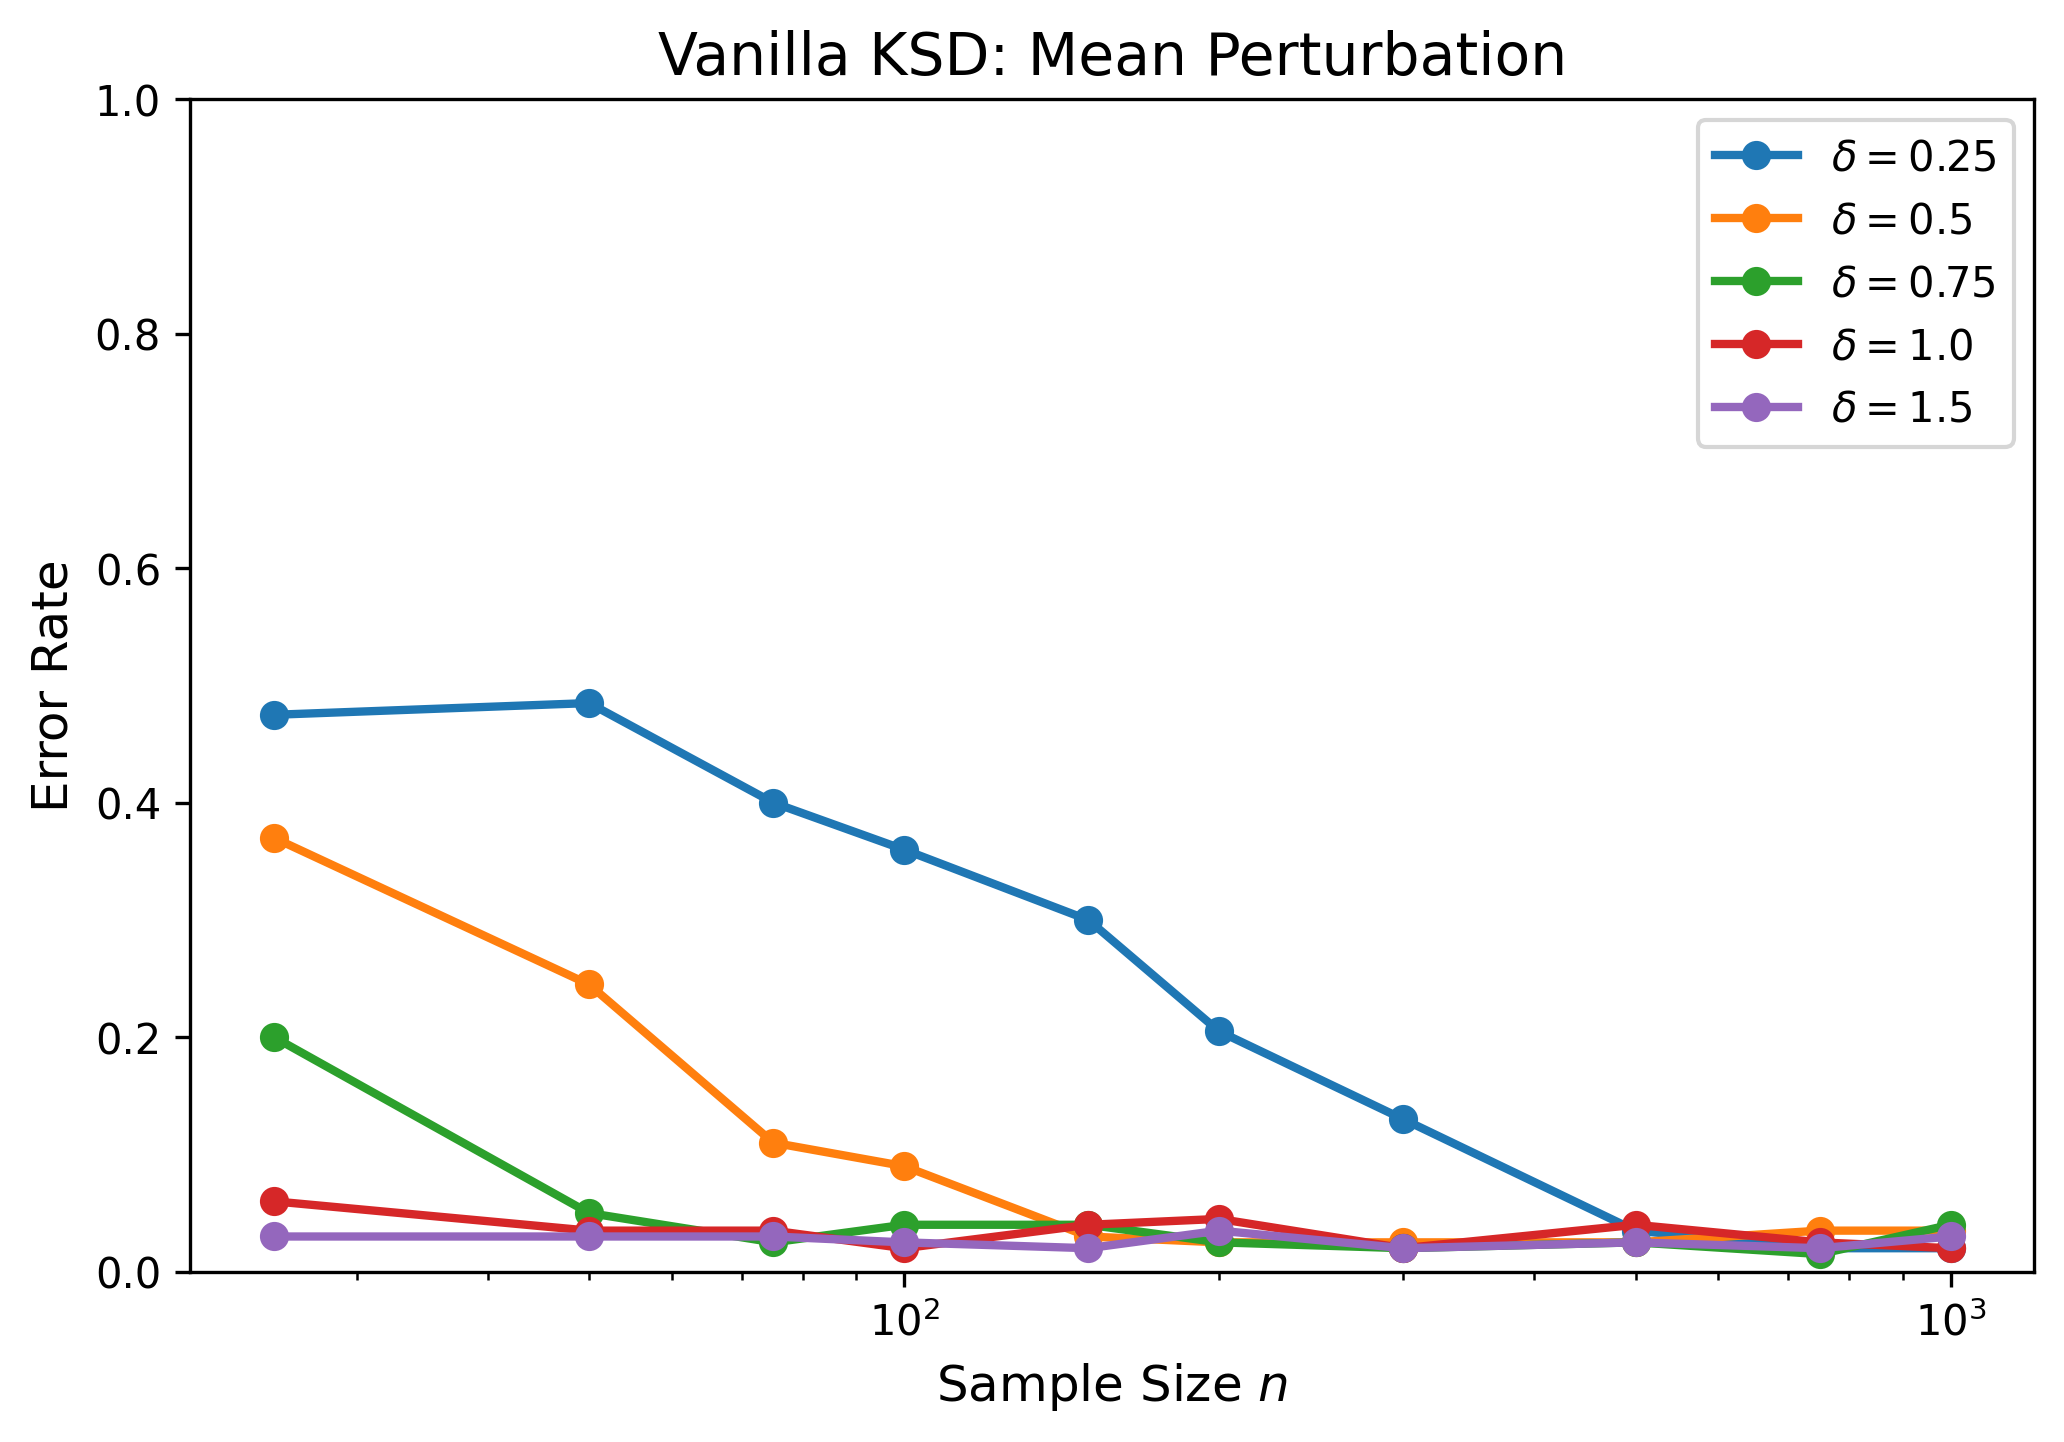
\includegraphics[width=0.47\textwidth]{KSD/Vanilla/vanilla_ksd_mean_perturbation_error_rate.png}
    \hspace{0.02\textwidth}
    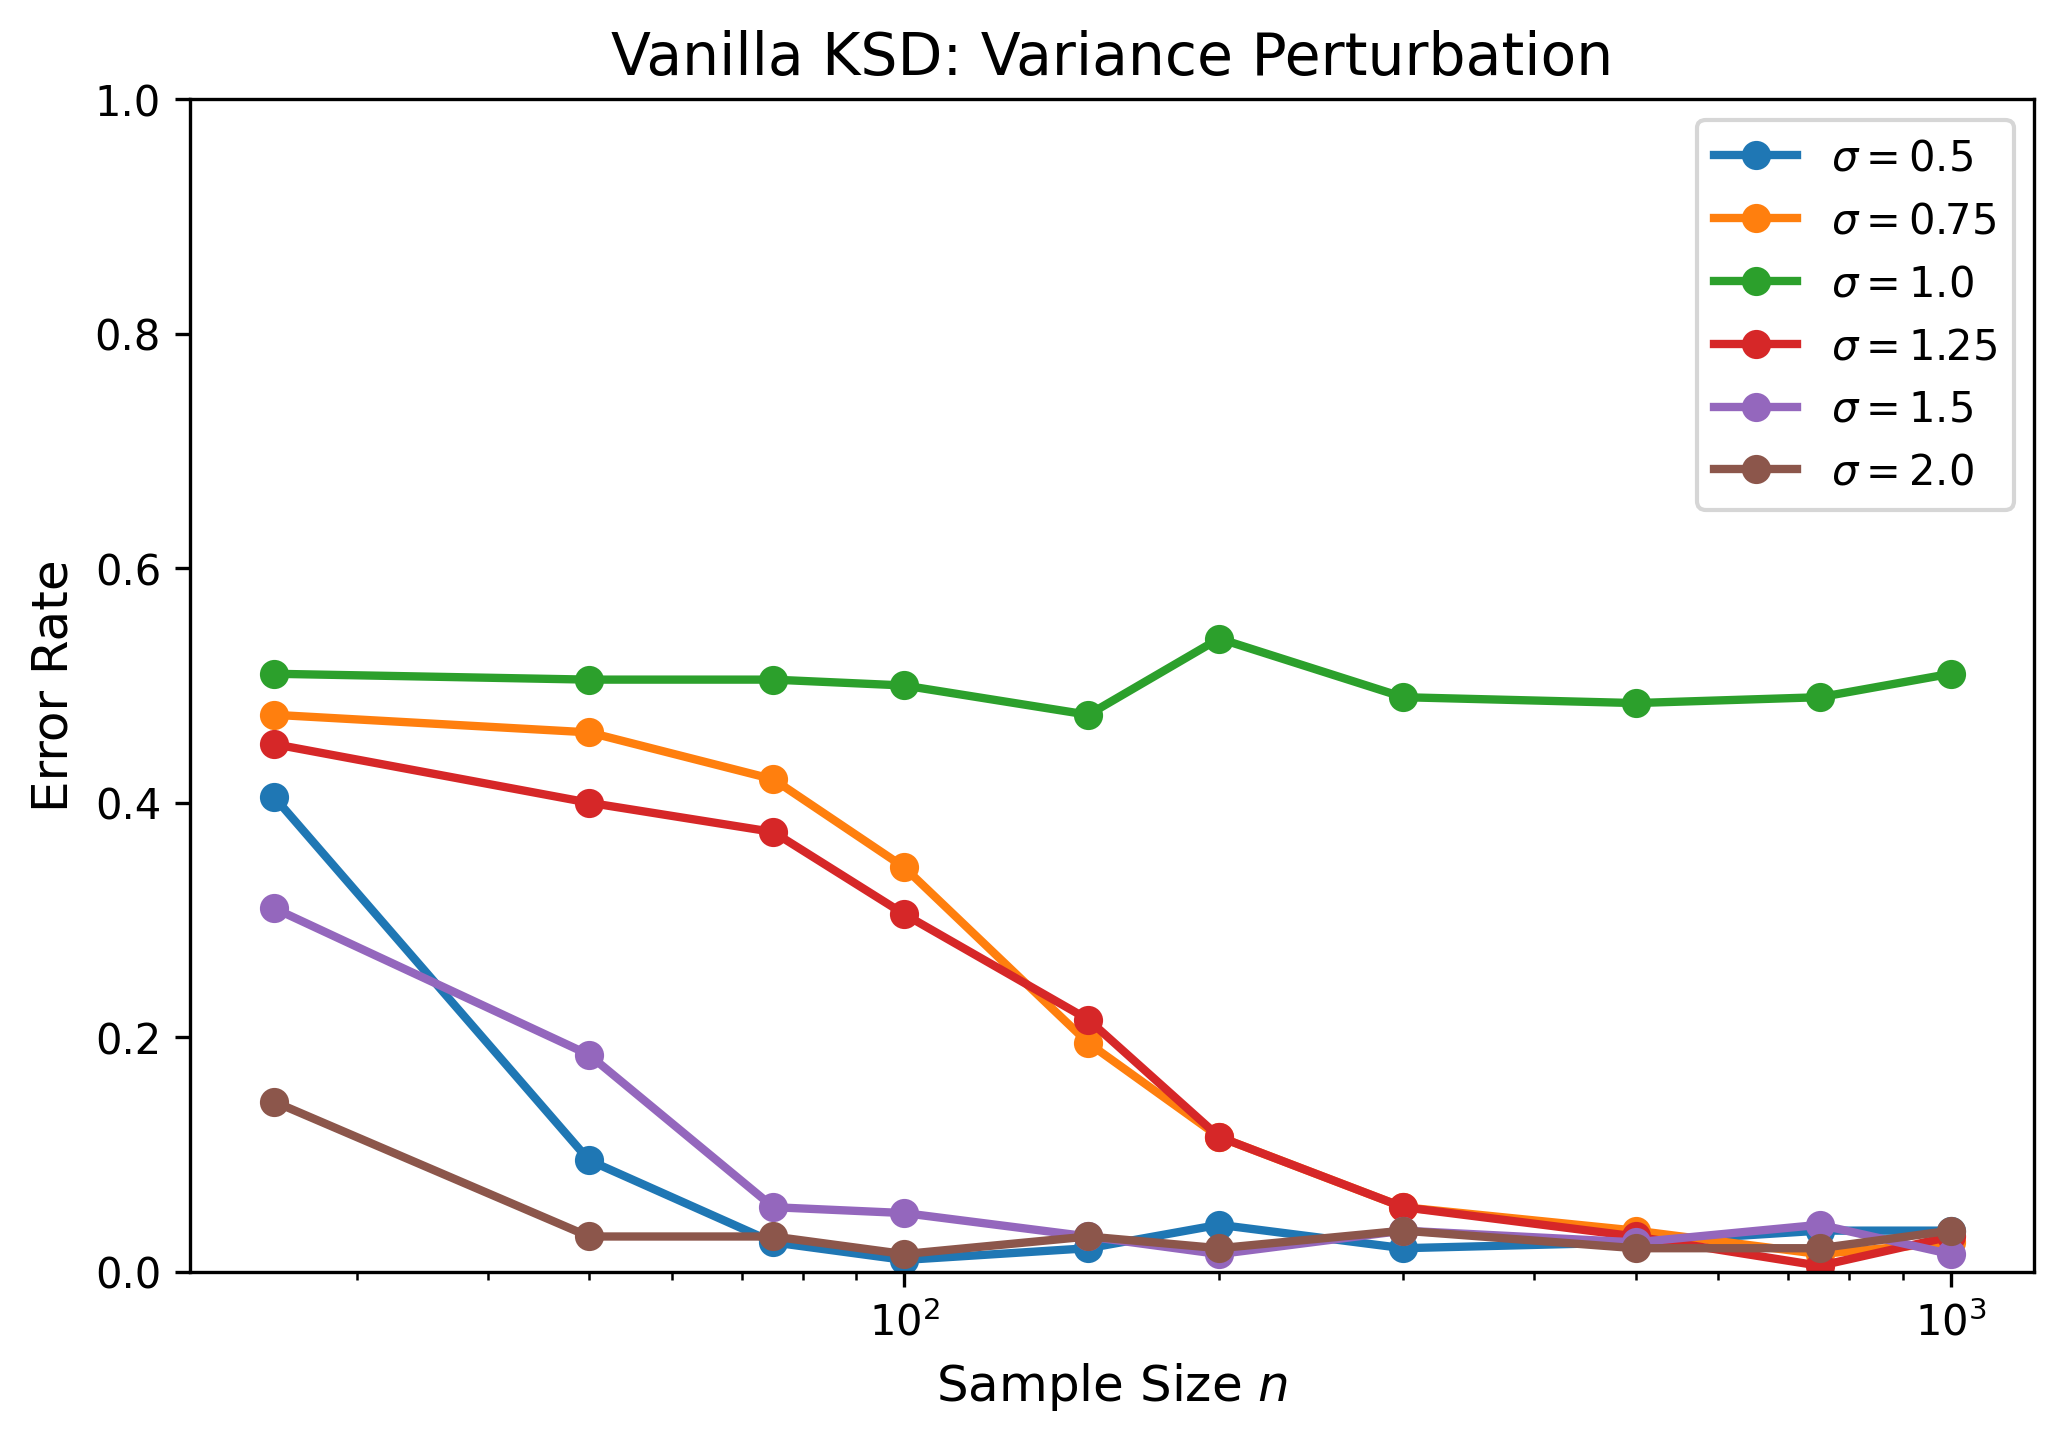
\includegraphics[width=0.47\textwidth]{KSD/Vanilla/vanilla_ksd_variance_perturbation_error_rate.png}
\end{center}
\textbf{Key observations}
\end{center}
\begin{itemize}
    \item High AUC for sufficiently large distributional perturbations.
    \item Error rate decreases with increasing sample size.
    \item Performance is close to random when the null and alternative coincide.
\end{itemize}
\end{frame}

\begin{frame}{Learning the Score Function}

\textbf{Why learn the score?}
Score is difficult to compute analytically for complex image distributions.

\textbf{Score Matching}
\begin{center}
\[
x_0
\quad\xrightarrow{\text{add noise}}\quad
x_t=x_0+\sigma_t z
\quad\xrightarrow{\text{score network}}\quad
s_\theta(x_t,t)
\]
\end{center}

where
\[
    z\sim\mathcal{N}(0,I).
\]

\vspace{0.1cm}

The conditional score is available analytically:

\[\nabla_{x_t}\log q_t(x_t|x_0)
=
-\frac{z}{\sigma_t}
\]

\vspace{0.15cm}

The network is trained using the score-matching objective:

\[\theta^*
=
\arg\min_\theta
\mathbb{E}
\left[
\sigma_t
\left\|
s_\theta(x_t,t)
+
\frac{z}{\sigma_t}
\right\|_2^2
\right]
\]
\end{frame}

\begin{frame}{KSD on MNIST}
\textbf{Experiment:}
\[
H_0:\text{Even MNIST}
\qquad\text{vs.}\qquad
H_1:\text{Odd MNIST}
\]
\begin{itemize}
    \item Score network trained on MNIST even digits.
    \item $\sigma=25$, with diffusion time $t$ tuned experimentally.
    \item $128$ samples, $200$ bootstrap samples, $100$ trials.
\end{itemize}

\vspace{0.1cm}
\begin{columns}[T]
\column{0.40\textwidth}
\centering
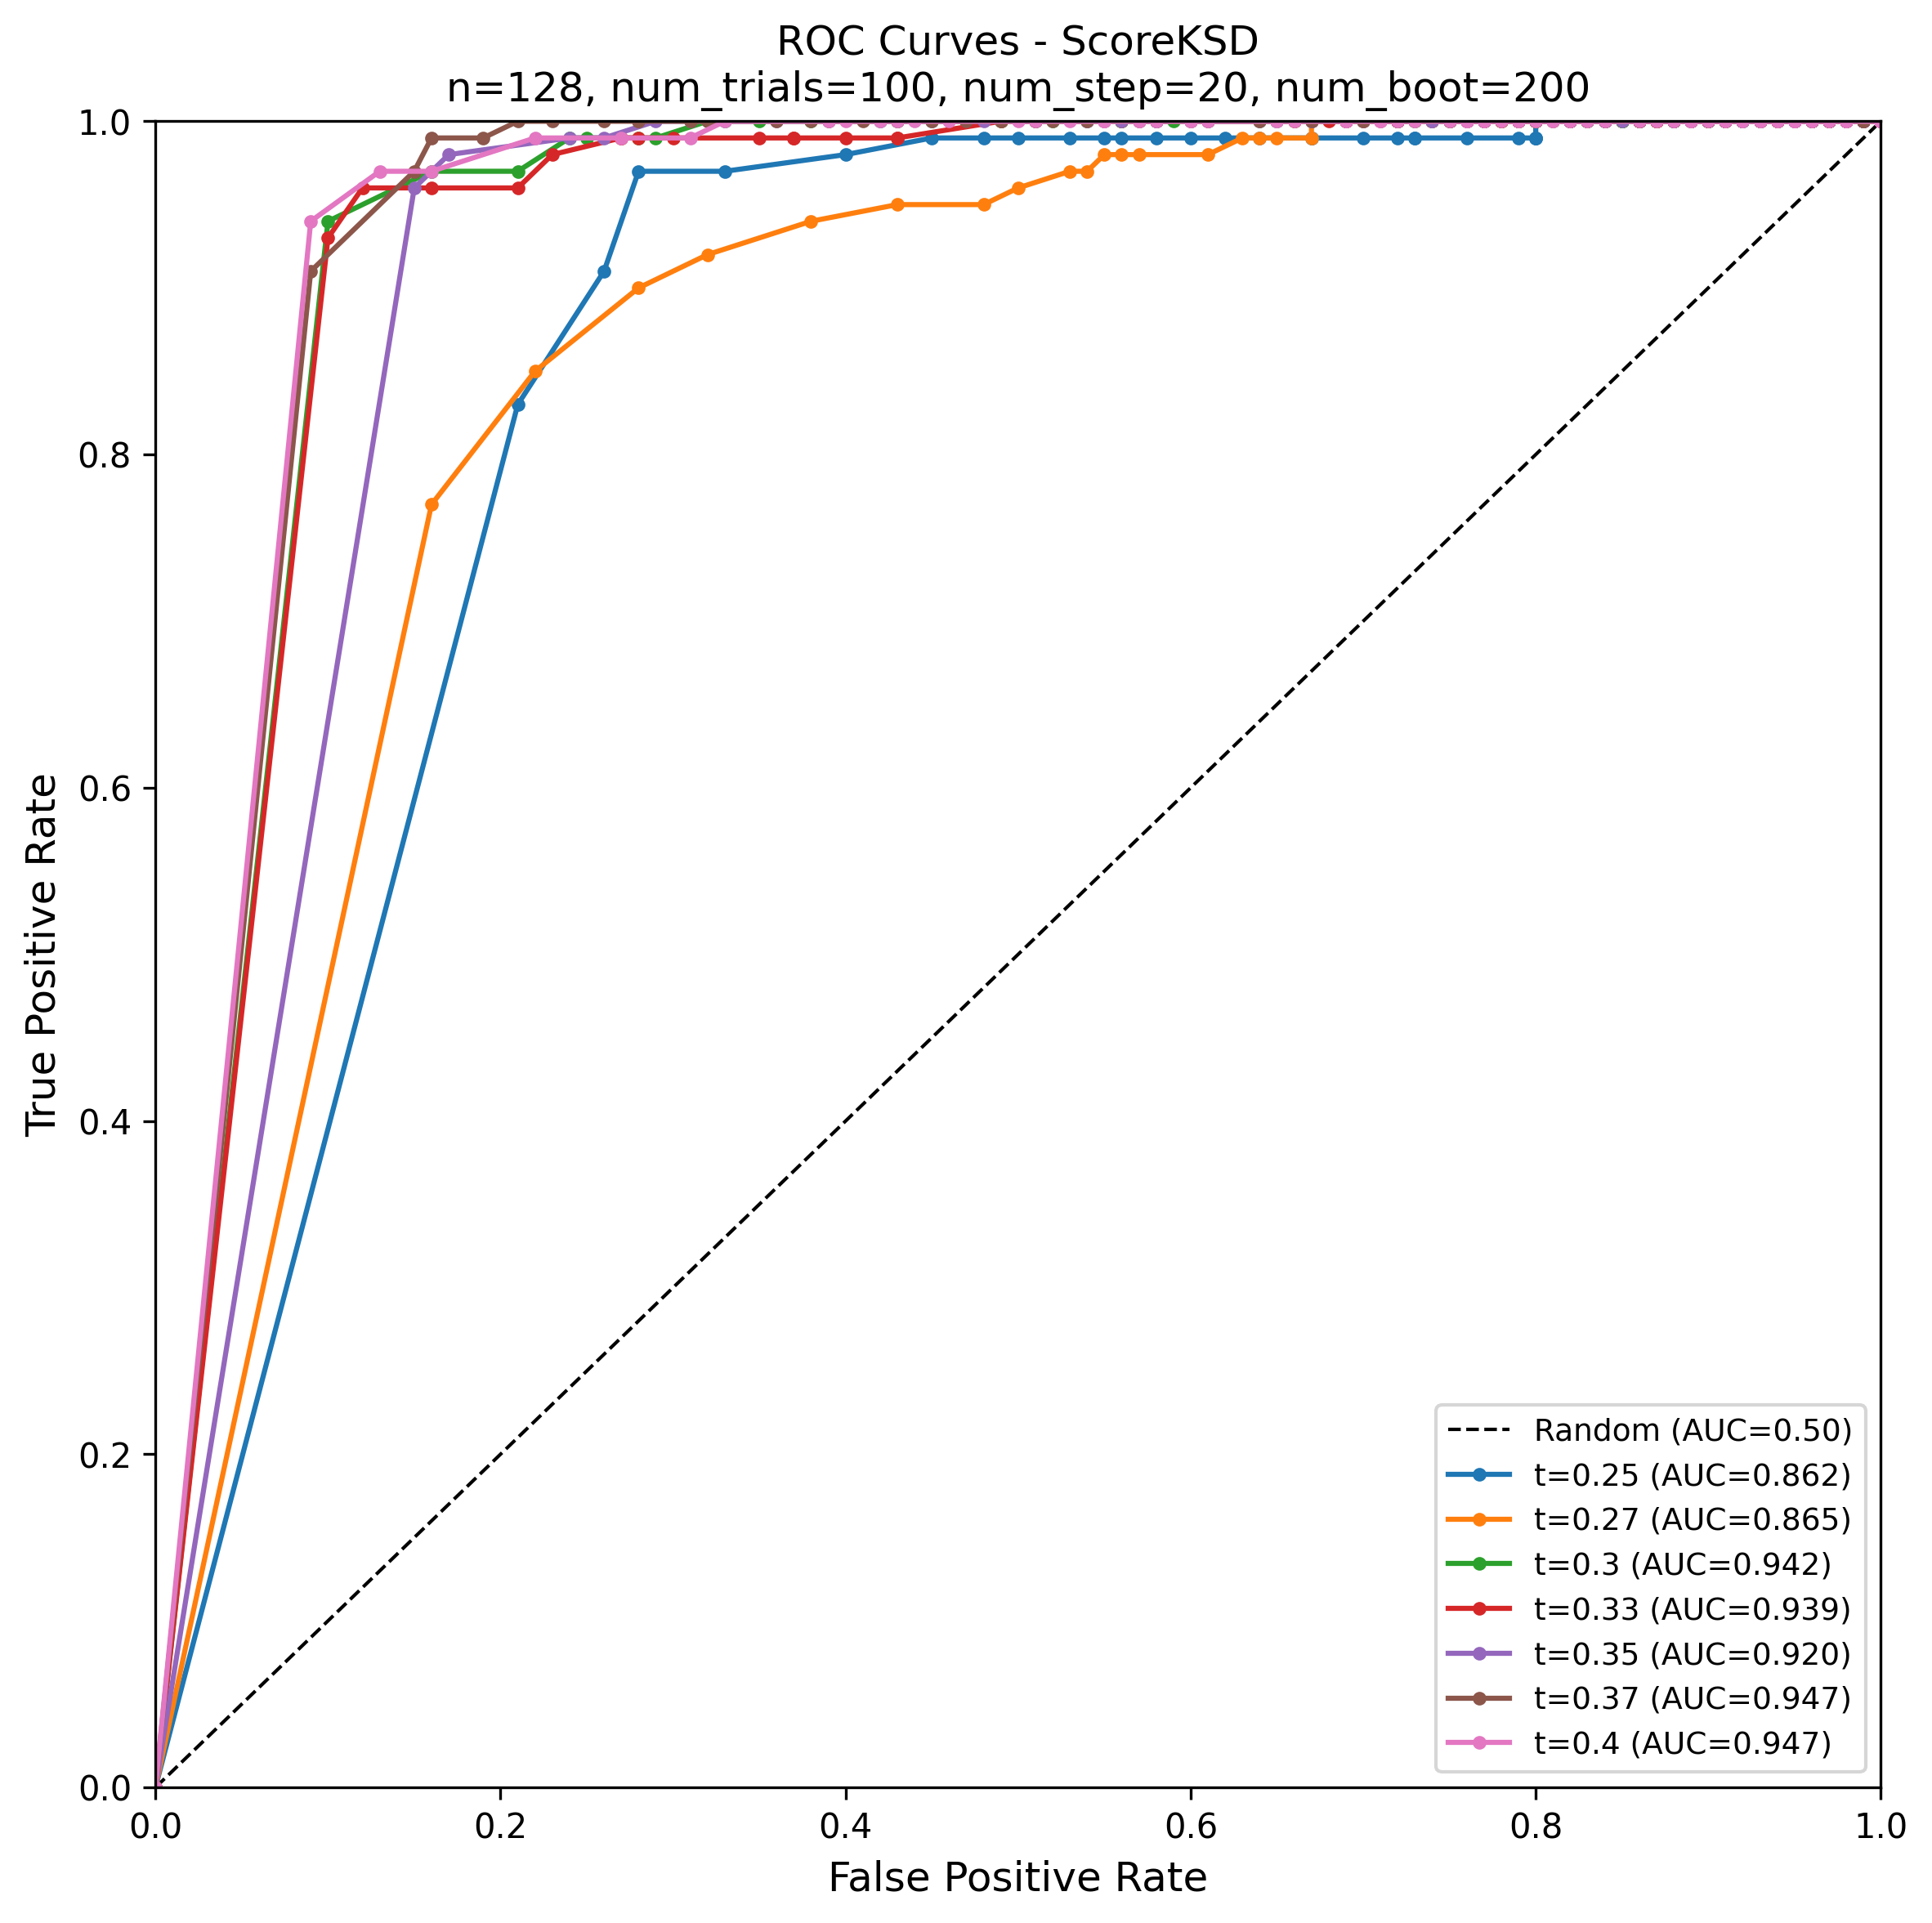
\includegraphics[width=\textwidth]{KSD/MNIST/roc_curve_scoreksd.png}
\column{0.40\textwidth}
\centering
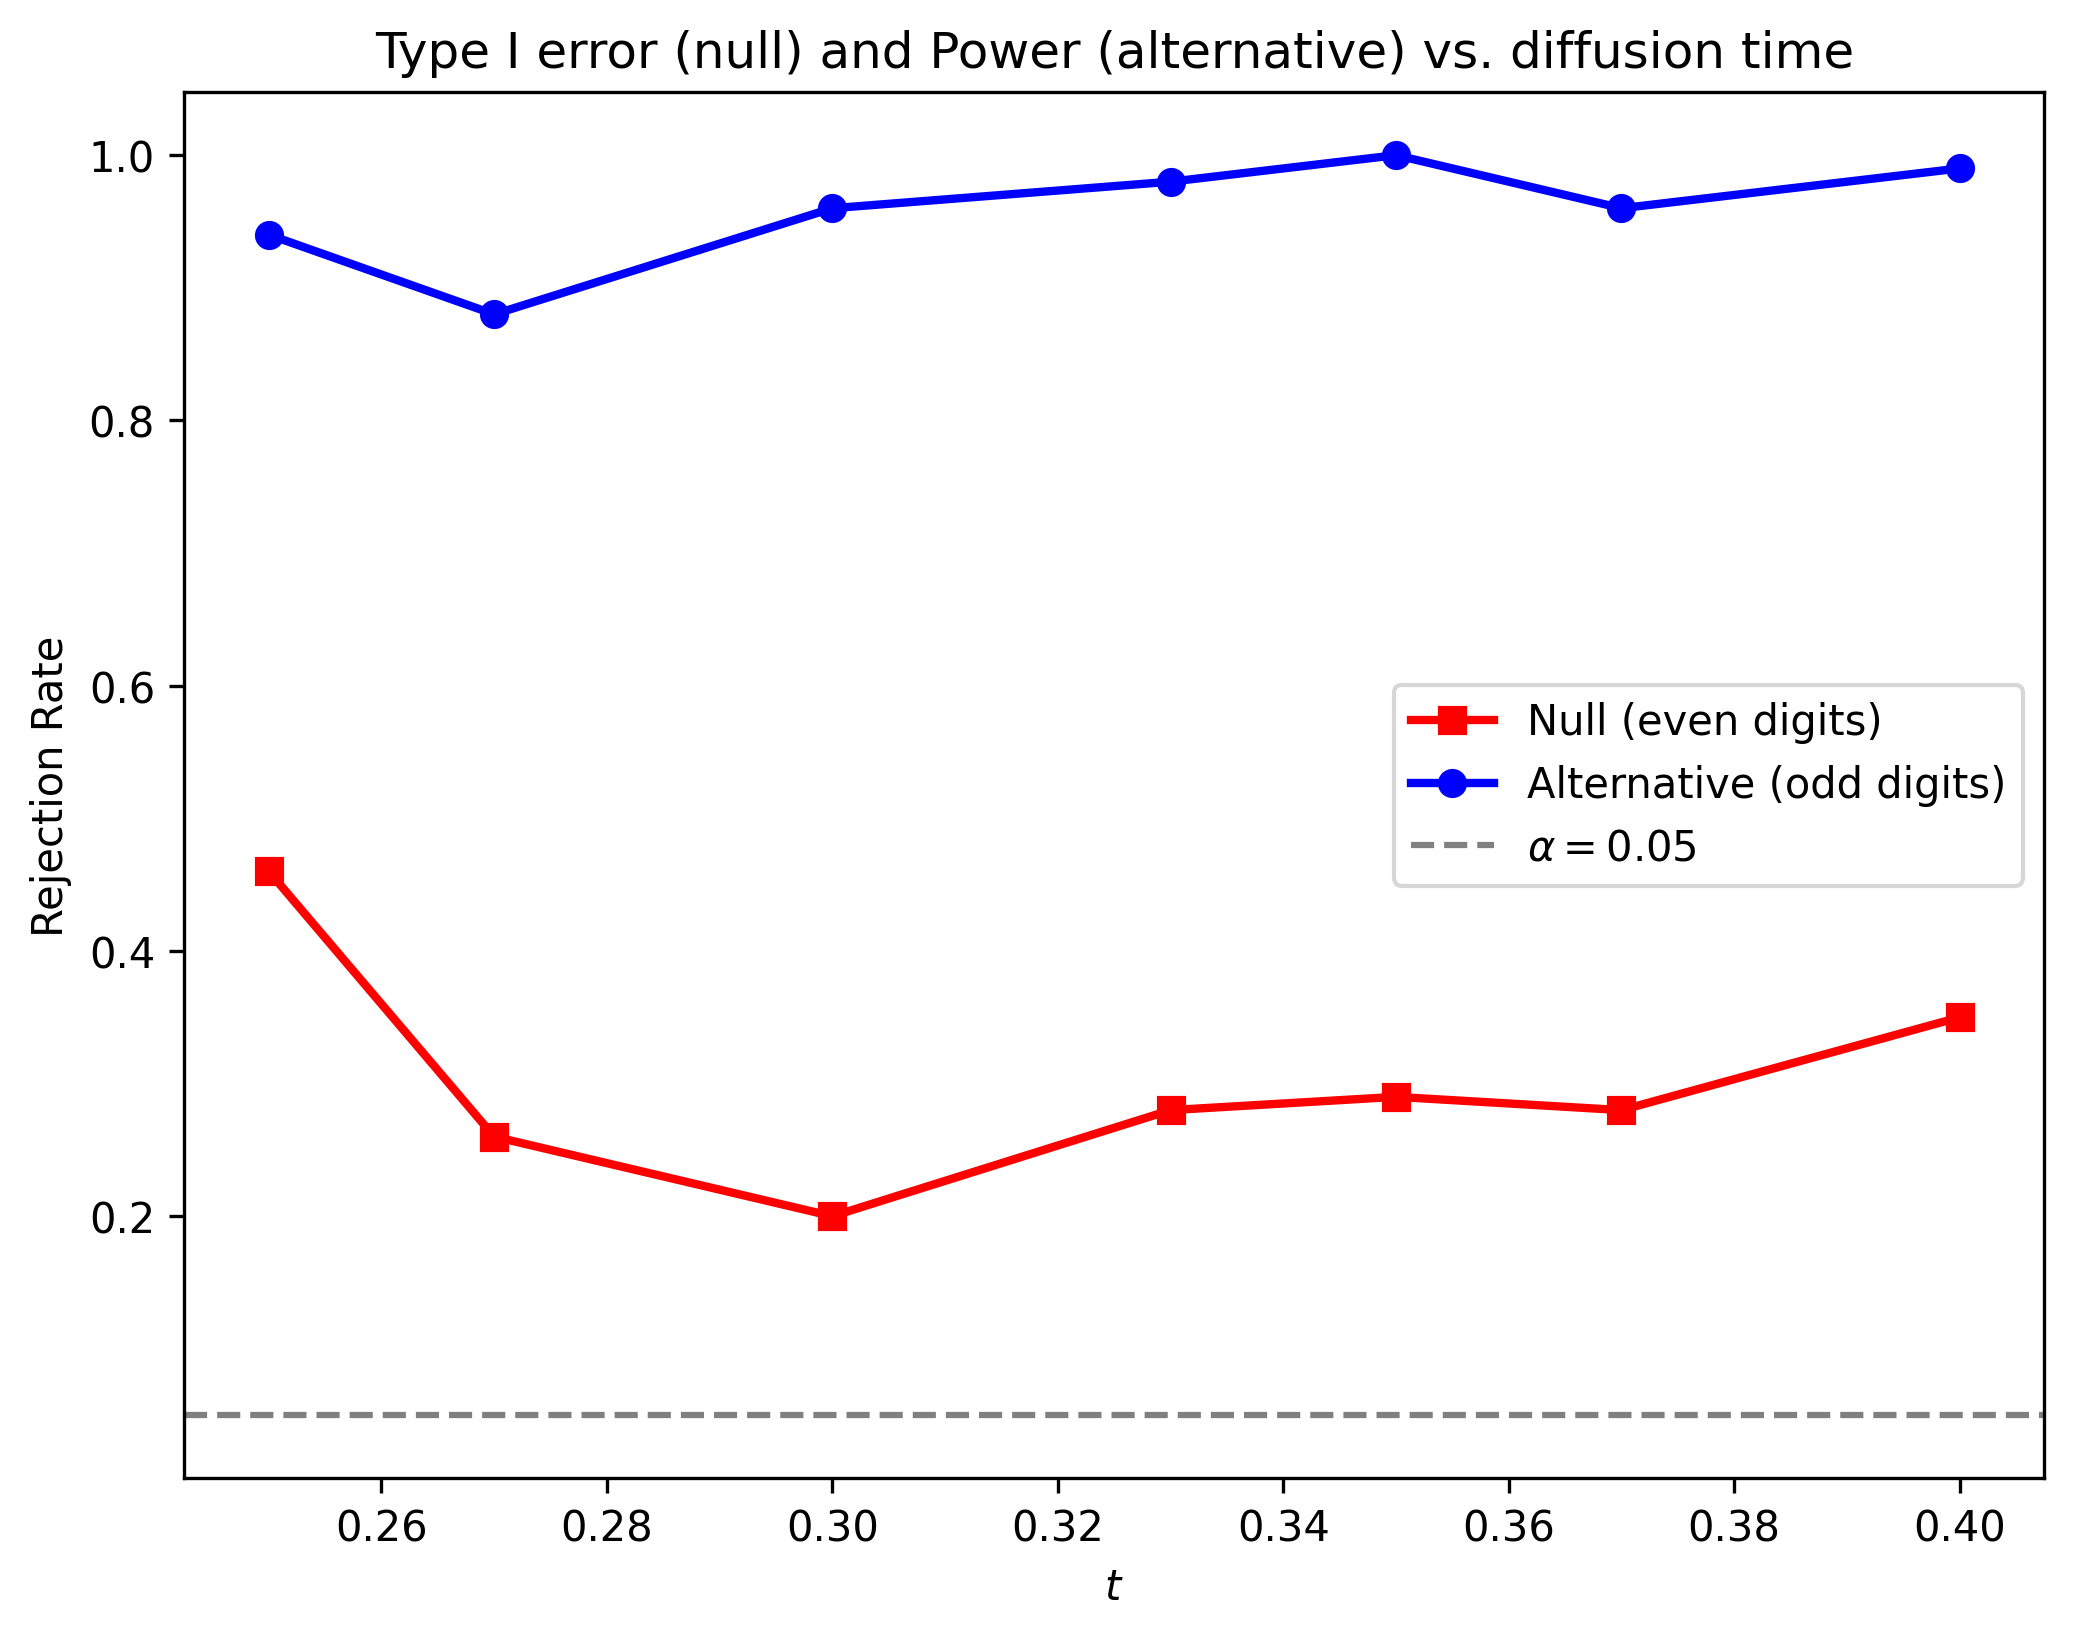
\includegraphics[width=\textwidth]{KSD/MNIST/combined_ksd_null_alt.png}
\end{columns}

\vspace{0.1cm}
\begin{center}
\textbf{Best AUC} $\approx 0.947$
\qquad
\textbf{Key issue:} limited statistical power
\end{center}
\end{frame}

\begin{frame}{Diffusion Posterior Sampling}

\textbf{Inverse problem}
\[
y=A(x_0)+\epsilon
\]

\begin{center}
\[
\text{Noisy observation }y
\quad\longrightarrow\quad
\text{Posterior samples }x_0
\]
\end{center}

\vspace{0.1cm}
\textbf{DPS with the learned score}
\begin{enumerate}
    \item Start from noisy sample $x_t$.
    \item Estimate the clean image using Tweedie's formula:
    \[
    \hat{x}_0=x_t+\sigma_t^2s_\theta(x_t,t).
    \]
    
    \item Measure consistency with the observation:
    \[
    L_{\mathrm{meas}}
    =
    \|y-A(\hat{x}_0)\|_2^2.
    \]
    
    \item Correct the reverse diffusion step:
    \[
    x_{t-dt}
    =
    x'_{t-dt}
    -
    \zeta_t\nabla_{x_t}L_{\mathrm{meas}}.
    \]
\end{enumerate}

\vspace{0.05cm}
\begin{center}
\textbf{Reverse SDE + measurement correction}
\end{center}
\end{frame}


\begin{frame}{DPS Reconstruction Results - I}
\textbf{Reconstruction settings}
\begin{itemize}
    \item Gaussian noise
    \item $20\%$ Inpainting
    \item Guidance parameter:
    $\zeta' \in \{0.001,0.005,0.01,0.05,0.1,0.5,1,5,10\}$
\end{itemize}

\vspace{0.1cm}

\begin{columns}[T,onlytextwidth]
    % Gaussian
    \column{0.48\textwidth}
    \centering
    {\large\bfseries Gaussian}
    \vspace{0.15cm}
    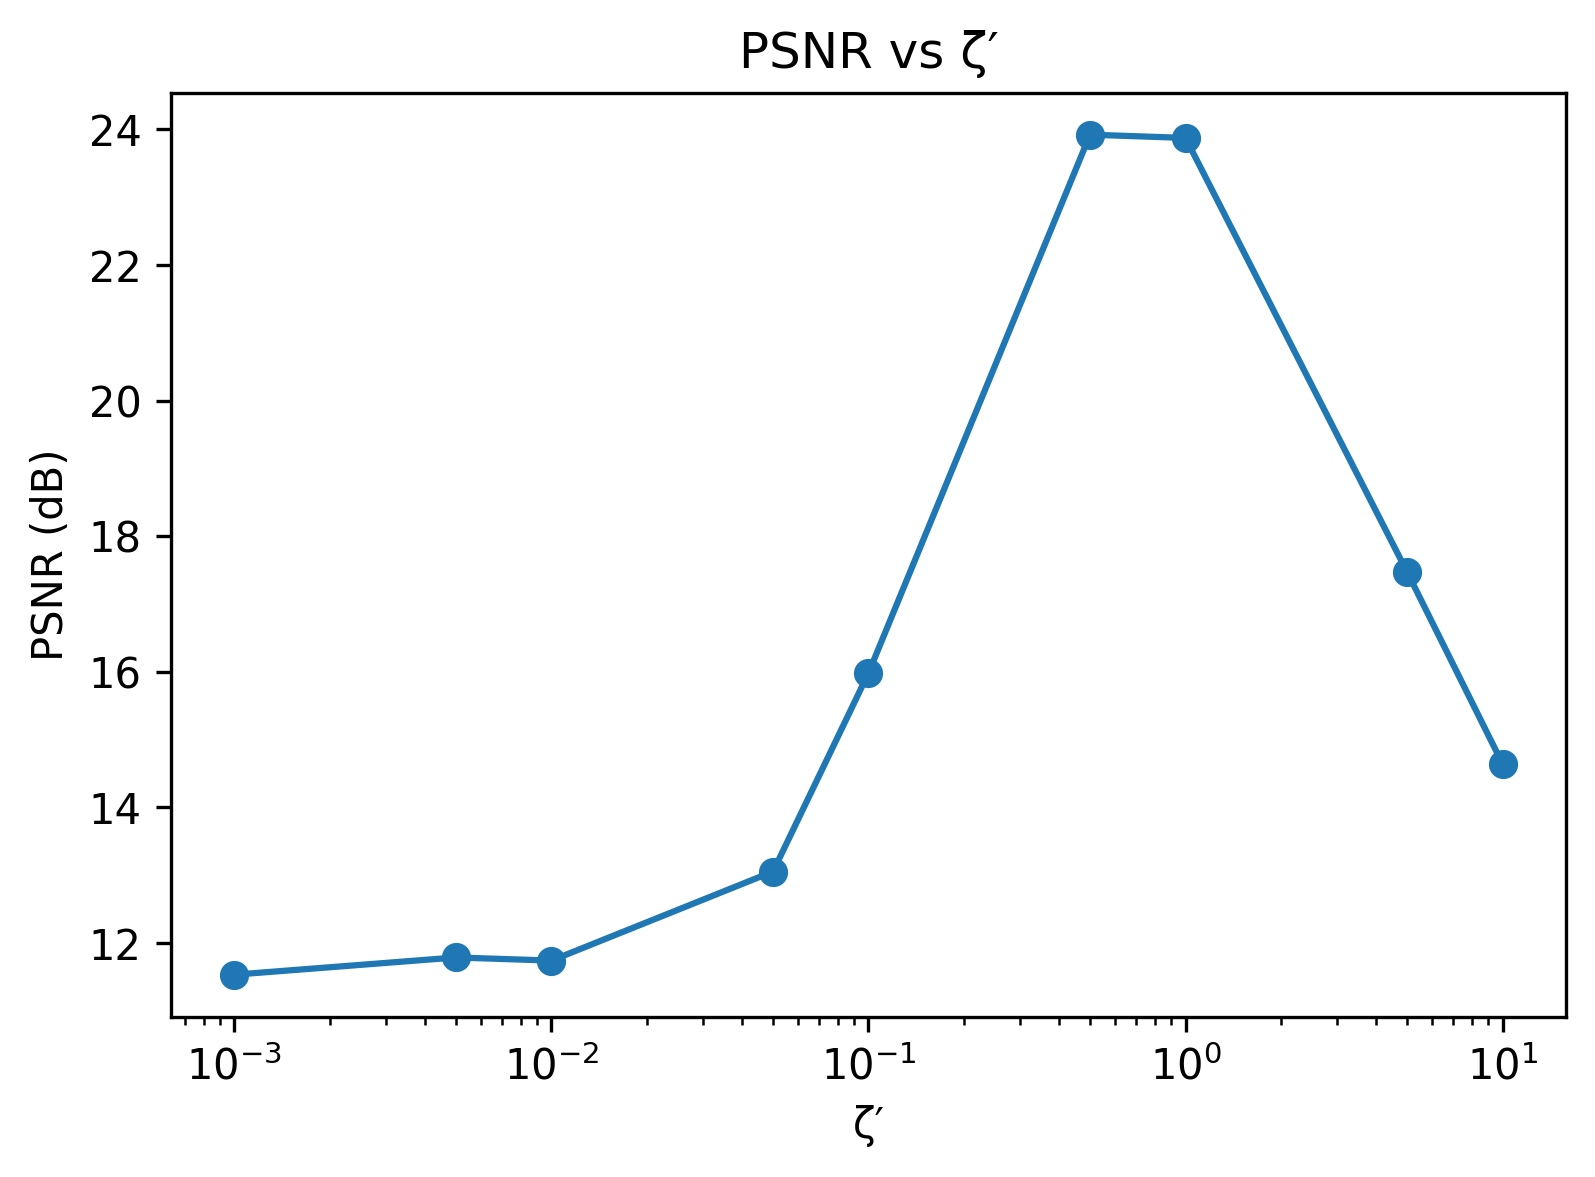
\includegraphics[
        width=\linewidth
    ]{DPS_VESDE/MNIST/Gauss/PSNR_Gaussian_dps.png}


    % Inpainting
    \column{0.48\textwidth}
    \centering
    {\large\bfseries Inpainting}
    \vspace{0.15cm}
    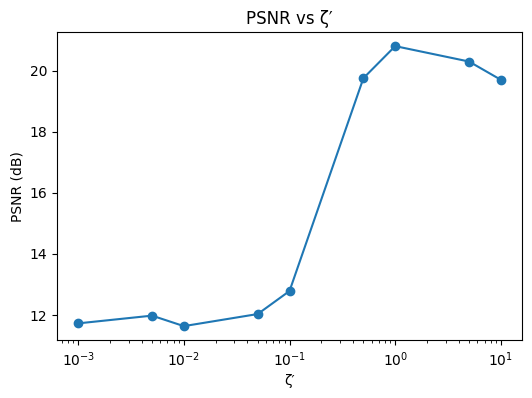
\includegraphics[
        width=\linewidth
    ]{DPS_VESDE/MNIST/Inpainting/PSNR_Inpainting_dps.png}
\end{columns}
\end{frame}

\begin{frame}{DPS Reconstruction Results - II}

\begin{center}

\textbf{\large Gaussian Noise}

\vspace{0.15cm}

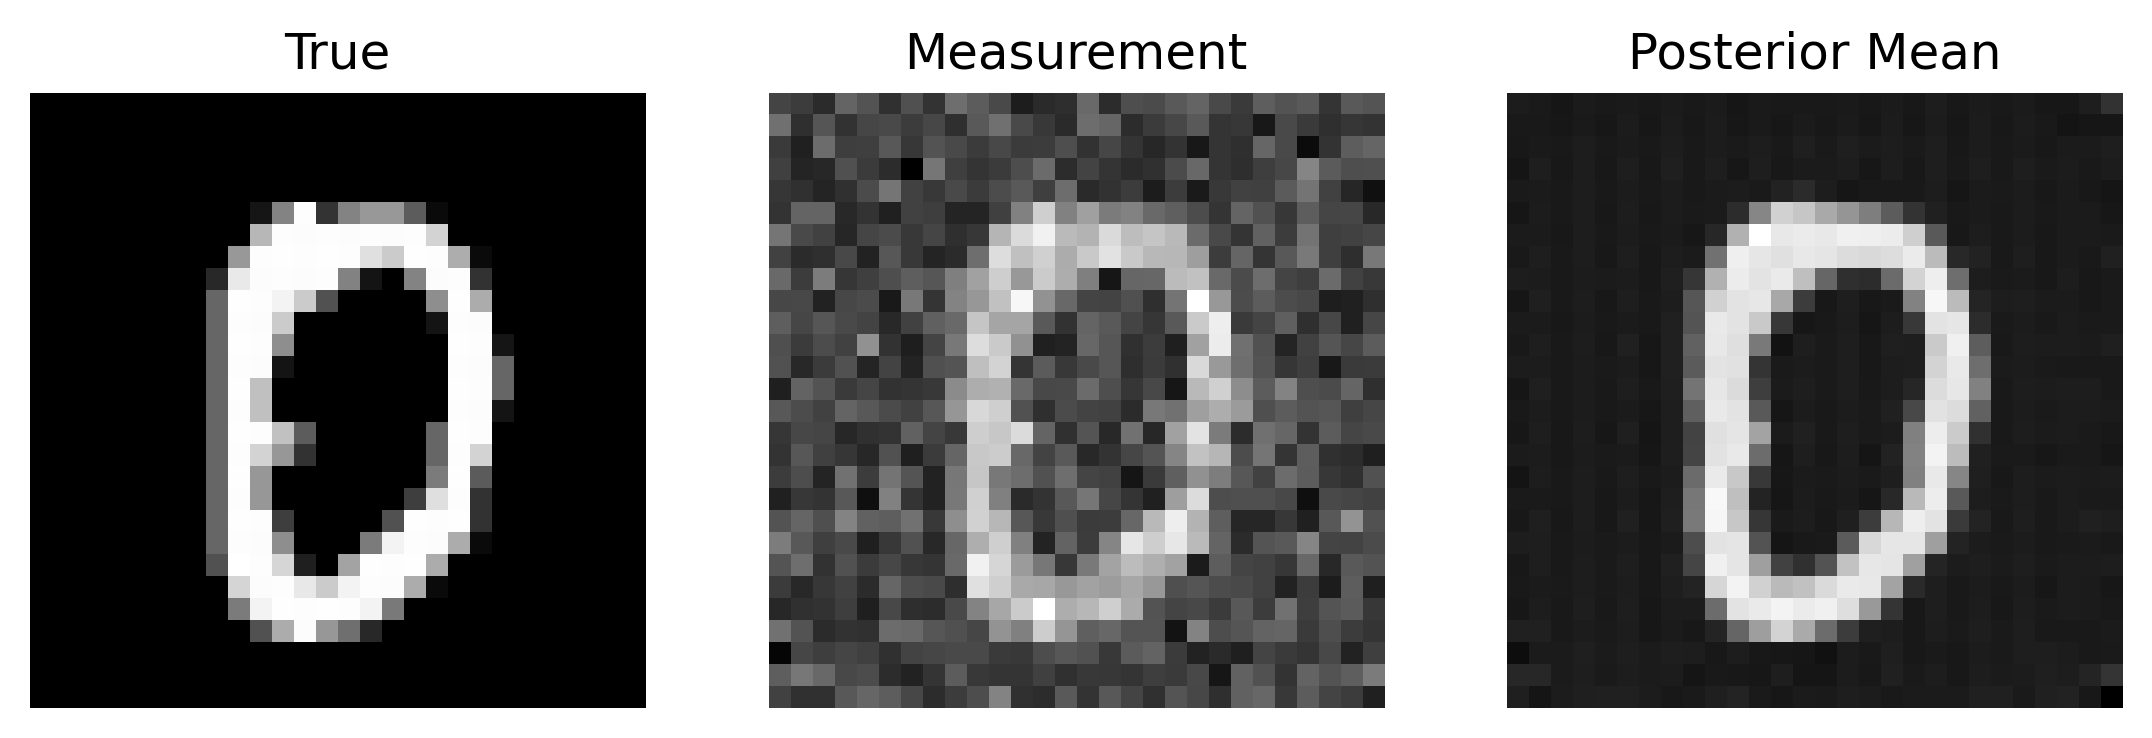
\includegraphics[width=0.75\textwidth]{DPS_VESDE/MNIST/Gauss/Gaussian_posterior_mean_single_digit.png}

\vspace{0.3cm}

\textbf{\large 20\% Inpainting}

\vspace{0.15cm}
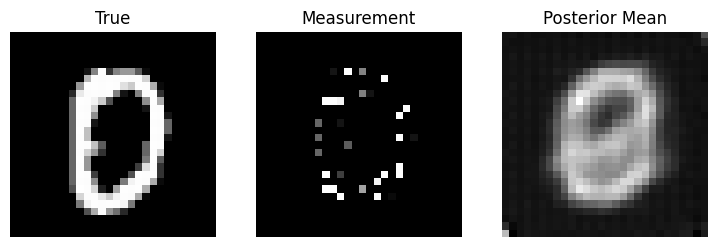
\includegraphics[width=0.75\textwidth]{DPS_VESDE/MNIST/Inpainting/Inpainting_posterior_mean_single_digit.png}

\end{center}
\end{frame}

\begin{frame}{DPS Reconstruction Results - III}

\begin{center}
\textbf{\large Gaussian Noise Different $\zeta'$}
\vspace{0.15cm}
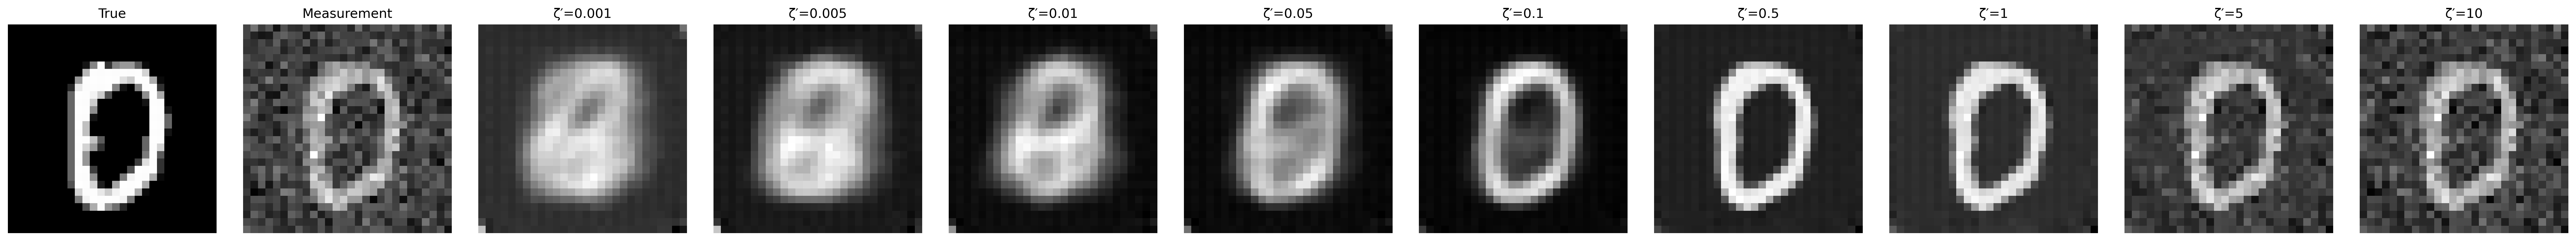
\includegraphics[width=0.95\textwidth]{DPS_VESDE/MNIST/Gauss/Gaussian_posterior_mean_different_zeta_prime.png}

\vspace{0.3cm}

\textbf{\large 20\% Inpainting Different $\zeta'$}
\vspace{0.15cm}
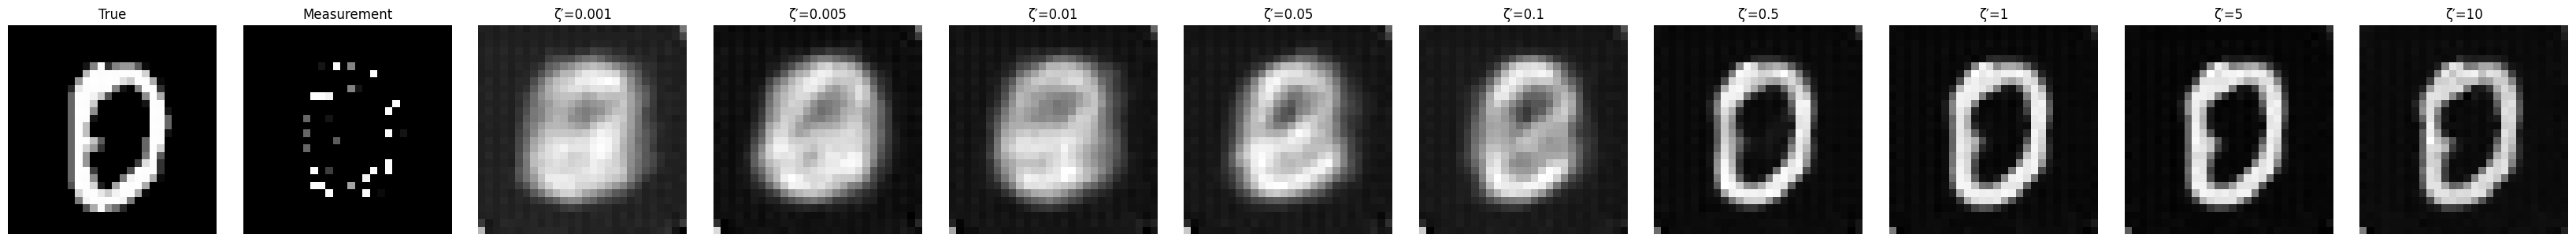
\includegraphics[width=0.95\textwidth]{DPS_VESDE/MNIST/Inpainting/Inpainting_posterior_mean_different_zeta_prime.png}

\end{center}
\end{frame}

\begin{frame}{KSD on Diffusion Posterior Samples}

\textbf{Goal:}
Test whether the generated DPS samples retain the statistical
properties required by the KSD framework.

\vspace{0.15cm}

\textbf{KSD Power Test}

\begin{center}

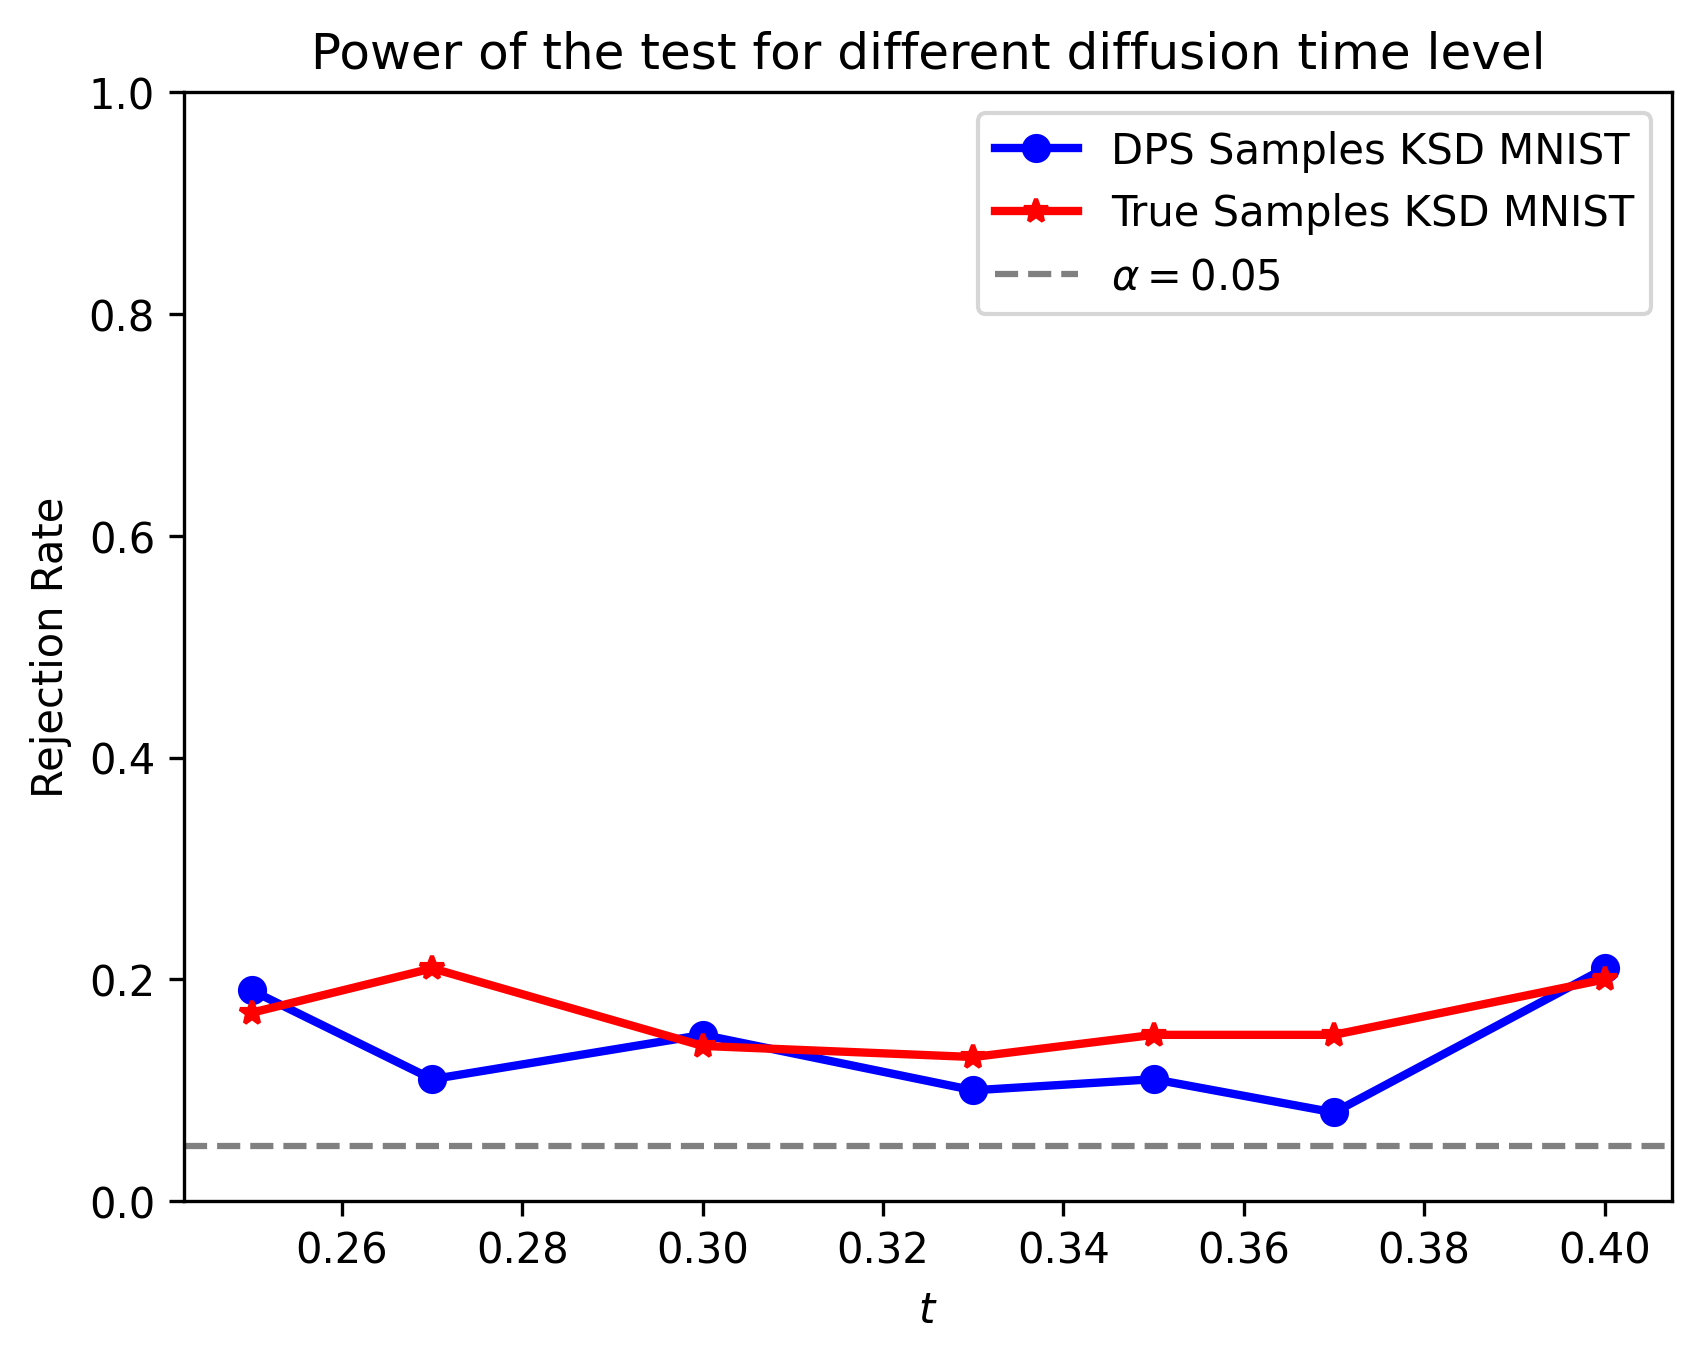
\includegraphics[width=0.5\textwidth]{DPS_VESDE/MNIST/Gauss/ksd_score_dps_gauss_even.png}

\end{center}

\vspace{0.1cm}

\begin{itemize}
    \item Compare KSD power for true samples and DPS samples.
    \item The overall power is similar for both cases.
    \item Statistical power is still below the desired level.
\end{itemize}
\end{frame}

\begin{frame}{Conclusion \& Future Work}
\textbf{What we achieved}
\begin{enumerate}
    \item \textbf{KSD-U}
    Effective goodness-of-fit testing on Gaussian toy examples.
    \item \textbf{Learned Score + KSD}
    Extended KSD to high-dimensional MNIST data using Score Matching.
    \item \textbf{DPS}
    Generated posterior samples for Gaussian noise and inpainting.
    \item \textbf{KSD + DPS}
    KSD power on DPS samples is comparable to that on true samples.
\end{enumerate}

\vspace{0.25cm}
\textbf{Future Work}
\begin{itemize}
    \item Learned kernels for improved statistical power.
    \item Perturbed kernels / Pooled KSD for multimodal settings.
    \item Comparison with MMD and other GoF methods.
\end{itemize}
\end{frame}

\begin{frame}{End}
\begin{center}
\vfill
{\Huge \textbf{Thank You}}
\vspace{0.5cm}
\end{center}

\begin{center}
{\Large Questions?}
\vfill
\end{center}
\end{frame}
\end{document}